% This is "sig-alternate.tex" V1.9 April 2009
% This file should be compiled with V2.4 of "sig-alternate.cls" April 2009
%
% This example file demonstrates the use of the 'sig-alternate.cls'
% V2.4 LaTeX2e document class file. It is for those submitting
% articles to ACM Conference Proceedings WHO DO NOT WISH TO
% STRICTLY ADHERE TO THE SIGS (PUBS-BOARD-ENDORSED) STYLE.
% The 'sig-alternate.cls' file will produce a similar-looking,
% albeit, 'tighter' paper resulting in, invariably, fewer pages.
%
% ----------------------------------------------------------------------------------------------------------------
% This .tex file (and associated .cls V2.4) produces:
%       1) The Permission Statement
%       2) The Conference (location) Info information
%       3) The Copyright Line with ACM data
%       4) NO page numbers
%
% as against the acm_proc_article-sp.cls file which
% DOES NOT produce 1) thru' 3) above.
%
% Using 'sig-alternate.cls' you have control, however, from within
% the source .tex file, over both the CopyrightYear
% (defaulted to 200X) and the ACM Copyright Data
% (defaulted to X-XXXXX-XX-X/XX/XX).
% e.g.
% \CopyrightYear{2007} will cause 2007 to appear in the copyright line.
% \crdata{0-12345-67-8/90/12} will cause 0-12345-67-8/90/12 to appear in the copyright line.
%
% ---------------------------------------------------------------------------------------------------------------
% This .tex source is an example which *does* use
% the .bib file (from which the .bbl file % is produced).
% REMEMBER HOWEVER: After having produced the .bbl file,
% and prior to final submission, you *NEED* to 'insert'
% your .bbl file into your source .tex file so as to provide
% ONE 'self-contained' source file.
%
% ================= IF YOU HAVE QUESTIONS =======================
% Questions regarding the SIGS styles, SIGS policies and
% procedures, Conferences etc. should be sent to
% Adrienne Griscti (griscti@acm.org)
%
% Technical questions _only_ to
% Gerald Murray (murray@hq.acm.org)
% ===============================================================
%
% For tracking purposes - this is V1.9 - April 2009

\documentclass{sig-alternate}
%\usepackage{longtable}
%\usepackage{caption}
\usepackage{graphicx}
\usepackage{caption}
\DeclareCaptionType{copyrightbox}
\usepackage{subcaption}
\usepackage{url}
%\usepackage{float}
%\usepackage{times}
%\usepackage{multirow}
%\usepackage{listings}
%\usepackage{times}
%\usepackage{paralist}
\usepackage{epsfig}
%\usepackage{subfigure}
%\usepackage{longtable}
\usepackage{hyperref}   
\hypersetup{colorlinks=false,urlcolor=blue}
\hypersetup{pdfborder={0 0 0}}
%\usepackage{subfigure}
\usepackage{color}
\usepackage[numbers]{natbib}
\usepackage{breakurl}
%\usepackage{ifpdf}
%\usepackage{wrapfig}
%\usepackage{float}
%\usepackage{texdraw}
%\usepackage{epsf}
%\usepackage{array}
%\usepackage{cite}
%\usepackage{enumitem}
%\usepackage{verbatim}
%\usepackage{setspace}
%\sloppy
%\usepackage{geometry}
%\usepackage{listings}
\usepackage{epstopdf}
\usepackage{grffile}


\newif\ifdraft
%\drafttrue
\ifdraft
\newcommand{\abhi}[1]{ {\textcolor{red} { ***Abhinav: #1 }}}
\else
\newcommand{\abhi}[1]{ {}}
\fi
%\newcommand{\ty}{\texttt}


\begin{document}
%
% --- Author Metadata here ---
\conferenceinfo{XSEDE}{'13 San Diego, CA USA}
%\CopyrightYear{2007} % Allows default copyright year (20XX) to be over-ridden - IF NEED BE.
%\crdata{0-12345-67-8/90/01}  % Allows default copyright data (0-89791-88-6/97/05) to be over-ridden - IF NEED BE.
% --- End of Author Metadata ---

\title{Making Campus Bridging Work for Researchers: \\A Case Study with mlRho}

%mlRho -- The Anatomy of a Successful Campus Bridging Project}
% \titlenote{(Produces the permission block, and
%copyright information). For use with
%SIG-ALTERNATE.CLS. Supported by ACM.}}
%\subtitle{[Extended Abstract]
%\titlenote{A full version of this paper is available as
%\textit{Author's Guide to Preparing ACM SIG Proceedings Using
%\LaTeX$2_\epsilon$\ and BibTeX} at
%\texttt{www.acm.org/eaddress.htm}}}
%
% You need the command \numberofauthors to handle the 'placement
% and alignment' of the authors beneath the title.
%
% For aesthetic reasons, we recommend 'three authors at a time'
% i.e. three 'name/affiliation blocks' be placed beneath the title.
%
% NOTE: You are NOT restricted in how many 'rows' of
% "name/affiliations" may appear. We just ask that you restrict
% the number of 'columns' to three.
%
% Because of the available 'opening page real-estate'
% we ask you to refrain from putting more than six authors
% (two rows with three columns) beneath the article title.
% More than six makes the first-page appear very cluttered indeed.
%
% Use the \alignauthor commands to handle the names
% and affiliations for an 'aesthetic maximum' of six authors.
% Add names, affiliations, addresses for
% the seventh etc. author(s) as the argument for the
% \additionalauthors command.
% These 'additional authors' will be output/set for you
% without further effort on your part as the last section in
% the body of your article BEFORE References or any Appendices.

\numberofauthors{6} %  in this sample file, there are a *total*
% of EIGHT authors. SIX appear on the 'first-page' (for formatting
% reasons) and the remaining two appear in the \additionalauthors section.
%
\author{
% You can go ahead and credit any number of authors here,
% e.g. one 'row of three' or two rows (consisting of one row of three
% and a second row of one, two or three).
%
% The command \alignauthor (no curly braces needed) should
% precede each author name, affiliation/snail-mail address and
% e-mail address. Additionally, tag each line of
% affiliation/address with \affaddr, and tag the
% e-mail address with \email.
%
% 1st. author
%Scientific Applications and Performance Tuning (SciAPT),\\
%                University Information Technology Services,\\ 
%                Indiana University, Bloomington, IN, 47408\\
\alignauthor
Abhinav Thota\\
%       \affaddr{Scientific Applications and Performance Tuning (SciAPT)},\\
%       \affaddr{               University Information Technology Services,}\\
       \affaddr{              Indiana University, Bloomington, IN, 47408}\\
       \email{athota@iu.edu}
% 2nd. author
\alignauthor
Scott Michael\\
%       \affaddr{Scientific Applications and Performance Tuning (SciAPT)},\\
%       \affaddr{               University Information Technology Services,}\\
       \affaddr{              Indiana University, Bloomington, IN, 47408}\\
       \email{scamicha@iu.edu}
% 3rd. author
\alignauthor 
Sen Xu\\
%       \affaddr{Scientific Applications and Performance Tuning (SciAPT)},\\
%       \affaddr{               University Information Technology Services,}\\
       \affaddr{              Indiana University, Bloomington, IN, 47408}\\
       \email{senxu@indiana.edu}
\and  % use '\and' if you need 'another row' of author names
% 4th. author
\alignauthor 
Bernhard Haubold\\
%       \affaddr{Scientific Applications and Performance Tuning (SciAPT)},\\
%       \affaddr{               University Information Technology Services,}\\
       \affaddr{              Max-Planck Institute for Evolutionary Biology, Pl\"{o}n, Germany}\\
       \email{haubold@evolbio.mpg.de}
% 5th. author
\alignauthor 
Thomas Doak\\
%       \affaddr{Scientific Applications and Performance Tuning (SciAPT)},\\
%       \affaddr{               University Information Technology Services,}\\
       \affaddr{              Indiana University, Bloomington, IN, 47408}\\
       \email{tdoak@indiana.edu}
% 6th. author
\alignauthor 
Robert Henschel\\
%       \affaddr{Scientific Applications and Performance Tuning (SciAPT)},\\
%       \affaddr{               University Information Technology Services,}\\
       \affaddr{              Indiana University, Bloomington, IN, 47408}\\
       \email{henschel@iu.edu}
}
% There's nothing stopping you putting the seventh, eighth, etc.
% author on the opening page (as the 'third row') but we ask,
% for aesthetic reasons that you place these 'additional authors'
% in the \additional authors block, viz.
% Just remember to make sure that the TOTAL number of authors
% is the number that will appear on the first page PLUS the
% number that will appear in the \additionalauthors section.

\maketitle
\begin{abstract}
  An increasing number of biologists' computational demands have outgrown the capacity of desktop
workstations and they are turning to supercomputers to run their simulations and calculations. Many of today's computational problems, however, require larger resource commitments than even individual universities can
 provide. XSEDE is one of the first places researchers turn to when they outgrow their campus
resources. XSEDE machines are far larger (by at least an order of magnitude) than what most universities offer. Transitioning from a campus resource to an XSEDE resource is seldom a trivial task. XSEDE has
  taken many steps to make this easier, including the Campus Bridging initiative, the Campus Champions
program, the Extended Collaborative Support Service (ECSS) \cite{ecss_web} program, and through education and outreach.

  In this paper, our team of biologists and application support analysts (including a Campus Champion) dissect a computationally intensive biology project and share the insights we gain
  to help strengthen the programs mentioned above. We worked on a project to calculate population mutation and
  recombination rates of tens of genome profiles using mlRho \cite{MEC:MEC4482}, a serial,
  open-source, genome analysis code. For the initial investigation, we estimated that we would need
  6.3 million service units (SUs) on the Ranger system. Three of the most important places where the biologists needed help in
  transitioning to XSEDE were (i) preparing the proposal for 6.3 million SUs on XSEDE, (ii) scaling up the
  existing workflow to hundreds of cores and (iii) performance optimization. The Campus Bridging initiative
  makes all of these tasks easier by providing tools and a consistent software stack across centers.

  Ideally, Campus Champions are able to provide support on (i), (ii) and (iii), while ECSS staff can assist
  with (ii) and (iii). But (i), (ii) and (iii) are often not part of a Campus Champion's regular job
  description. To someone writing an XSEDE proposal for the first time, a link to the guidelines and a few
  pointers may not always be enough for a successful application. In this paper we describe a new role for a
  campus bridging expert to play in closing the gaps between existing programs and present mlRho as a case study.
\end{abstract}

% A category with the (minimum) three required fields
\category{H.4}{Information Systems Applications}{Miscellaneous}
%A category including the fourth, optional field follows...
\category{D.2.8}{Software Engineering}{Metrics}[complexity measures, performance measures]

\terms{PERFORMANCE, EXPERIMENTATION}

\keywords{high-throughput, XSEDE, BigJob, pilot-job, genetics, mlRho, performance tuning, optimization}

\section{Introduction}
As first defined by the National Science Foundation Advisory Committee for Cyberinfrastructure's Task Force on Campus Bridging \cite{nsf2011}, and later expanded upon by \citeauthor{stewart2012}, campus bridging is:

\begin{quotation}
``...the seamlessly integrated use of cyberinfrastructure operated by a scientist or engineer
with other cyberinfrastructure on the scientist's campus, at other campuses, and at the regional, national,
and international levels as if they were proximate to the scientist, and when working within the context of a
Virtual Organization (VO) make the 'virtual' aspect of the organization irrelevant (or helpful) to the work of
the VO. \cite{stewart2012}''
\end{quotation}

In applying this definition of campus bridging to XSEDE, one of the biggest challenges for researchers moving
from campus resources to XSEDE resources is being able to scale up their workflows so that they are efficient
and can achieve high throughput on the larger XSEDE machines. While \citeauthor{stewart2012} identify key use
cases where campus bridging tools can improve a researcher's experience using XSEDE resources, one aspect that
is not included in their analysis is the dramatic increase in complexity that is inherent in the computational
and data storage systems when a researcher moves from his workstation to an XSEDE resource. This scale up in
complexity is in many cases a daunting prospect for a researcher new to XSEDE, who may have relatively little
computational experience. Even savvy users who have experience with campus clusters can encounter issues when
scaling up to XSEDE resources.

This challenge is distinct from the challenge of providing a canonical software stack, but can be compounded
by widely divergent software environments between campus and XSEDE resources. Even when the operating
environment is not very different on XSEDE resources, compared to campus resources, researchers can face
challenges with the sheer scale and complexity of XSEDE resources. In the situation described in this paper,
campus bridging included helping the researchers redesign their experiments and scale up their workflows to
move effectively from their local workstations to IU's modest sized cluster environment, and then on to using
the much larger XSEDE machines at Texas Advanced Computing Center (TACC). It should be noted that, in general, the differences in software
environment between the IU campus resources and the TACC supercomputers were superficial; the real challenges
lie in scaling up the applications and navigating the complexity of a much larger system.

In this paper we propose a new role for a campus bridging expert to help address the challenges
faced by researchers when moving from their workstation to XSEDE resources. A campus bridging expert helps
to bridge the gap between domain science and computer science and helps researchers
   move their applications from small-scale campus resources to much larger XSEDE resources. A campus
bridging expert is mostly a technologist, who is able to apply many different approaches to scaling up
applications, but should also be familiar with the common challenges of the scientific domain. The campus bridging expert must be able to
communicate effectively about XSEDE resources with researchers who may have little or no supercomputing experience. The
campus bridging expert role is distinct from the current Campus Champion and the role filled by the Extended
Collaborative Support Service (ECSS) team. As the name implies, the campus bridging expert closes the gap
between the Campus Champion role -- which is designed to provide information, guidance, and facilitate access
to XSEDE resources, and the ECSS role, which is designed to provide in-depth analysis, insight and development
for a particular scientific or engineering challenge. The role of campus bridging expert may, in fact, be
filled by the same people who are currently Campus Champions or ECSS team members; in many ways the functions
of the campus bridging expert are an extension of ECSS and Campus Champion functions. In this paper we discuss
how, by filling the role of campus bridging expert, we were able to bridge the gap between many different
sized resources and help researchers in the field of population genomics use some of the largest XSEDE
resources to conduct a research program at an unprecedented magnitude.

Researchers in the Indiana University (IU) Department of Biology have been conducting studies into population
genomics and evolution for some time. A newly developed computer program called mlRho \cite{MEC:MEC4482} is
being used to study ecological and genetic parameters in different populations. While mlRho is a serial code,
the investigation we have conducted with our XSEDE allocation was embarrassingly parallel in nature. The work
for each species was divided among many computational processes. To manage hundreds of processes for each of
the 40+ species of interest, we used the SAGA BigJob pilot-job tool \cite{bigjob_web}, which is
currently available on many XSEDE resources. BigJob allowed us to distribute the analyses for each species
across thousands of processor cores, depending on the genome sizes. Thus far we have
investigated a total of 46 individual genomes. In addition
to the use of the BigJob tool, we have done an extensive performance analysis of the mlRho code and have been able to improve the runtime of the code by a
factor of more than 50.

The remainder of the paper is organized as follows: section \ref{sec:background} gives some insight into the
computational methodologies and principles of biology being explored by the mlRho code. Section
\ref{sec:resources} outlines our initial estimates for the computational resources necessary to accomplish the
research agenda and the steps that were taken to secure an XSEDE allocation. In section \ref{sec:optimization},
we describe how, through tracing and profiling of the code, we were able to successfully optimize it and
dramatically increase its performance. Section \ref{sec:results} details the current status of the research
program and initial scientific results and in section \ref{sec:conclusion} we present conclusions.


\section{Scientific Background}\label{sec:background}
The amazing biodiversity on our planet has fascinated humans for thousands of years. To understand how this diversity arises and is maintained, it is critical to determine fundamental ecological and genetic parameters (e.g., population sizes, recombination rates) for a range of species. These parameters play important roles in creating opportunities for increasing genetic diversity, population divergence, and speciation. mlRho is a software package which uses next-generation genomic sequencing to generate a novel measure of linkage disequilibrium. Deploying mlRho on XSEDE resources has allowed us to study these important population-genetic parameters in a broad assembly of eukaryotic genomes.

Although there are several methods for determining recombination rates, they can be both time and resource intensive. The mlRho software employs a novel analytic approach that uses a new metric called the zygosity correlation coefficient, which is estimated using maximum likelihood (ML) methods. It only requires single individual genome sequences, but is extremely data intensive. Using mlRho and XSEDE computational resources, we have been able to examine the recombination rates of a plethora of species with accuracy that was previously unachievable. 

%Understanding how the amazing biodiversity on our planet has arisen is a biological question that has
%fascinated humans for thousands of years. It is critical to investigate the fundamental ecological and genetic
%parameters (e.g., population sizes, recombination rates) to disentangle the evolutionary process of the
%existing organisms. The ecological and genetic parameters play important roles in creating opportunities for
%increasing genetic diversity, population divergence, and speciation. Deploying mlRho, a software package which
%generates a novel measure of recombination rates, on XSEDE resources has allowed us to study these
%important population-genetic parameters in a broad assembly of eukaryotic species. This approach has been
%particularly fruitful when applied to the newly available genome sequences now being produced by
%next-generation sequencing methods.
%
%Although there are several methods for determining recombination rates, they can be both time and resource
%intensive. The mlRho software employs a novel analytic approach that uses a new metric called the zygosity
%correlation coefficient, which is estimated using ML. This approach requires single individual
%samples, but is extremely data intensive. Using the ML approach implemented in the mlRho software %developed at
%%IU and the Max Planck Institute for Evolutionary Biology in Germany, 
%and XSEDE computational resources, we have been able to examine the recombination rates of a plethora of
%species with accuracy that was previously unachievable.

\subsection{Program Description}
The mlRho software is a serial program that estimates mutation, recombination, and sequencing error rates from
genome sequences~\cite{MEC:MEC4482}. The underlying data consists of assembled sequencing reads obtained from
a single diploid individual. Such data are collected, for example, for the 1000 human genome project. mlRho reads a profile consisting of the number of each nucleotide (\texttt{A}, \texttt{C}, \texttt{G}, and \texttt{T}) from a file at each sequenced position.
   Given a mutation and error rate, mlRho computes two probabilities for each profile: The
probabilities of observing the profile given that the position is either mutated (heterozygous), or not
(homozygous). These probabilities depend on the mutation and error rates. By varying them, mlRho finds the
values that maximize the overall likelihood of the data.

While mutation and sequencing error affect individual genome positions, recombination uncouples the
evolutionary history of pairs of positions. This is observable as a decorrelation of the zygosity states between
pairs of positions. To estimate recombination, mlRho computes the probability of observing profile pairs
separated by, say, 1000 nucleotides. This is a function of the recombination rate and the single position
likelihoods.

\subsection{Linkage Disequilibrium and Recombination Rate}\label{sec:LD}
Linkage disequilibrium (LD), i.e., the non-random association of alleles at two or more loci, is an important
parameter for many areas of population genetics.  In recent years, there has been growing interest in
measuring LD across a broad range of species, because a proper understanding of LD would greatly facilitate
identifying the genetic loci which underlie important phenotypic variation in natural populations, as well as
human diseases. More importantly, LD is a population-genetic property that can help ascertain recombination
rate, because recombination is the primary evolutionary force that breaks down LD among genetic loci. Although
a substantial body of research has been devoted to elucidating the evolutionary consequences of
recombination~\cite{resolving-paradox}, the forces that determine recombination rates remain poorly
understood. For example, we have little idea what determines the occurrence of recombination on a chromosome,
what impact local DNA polymorphism has on recombination processes, and how recombination rates change over
evolutionary time~\cite{stumpf}.

Conventional approaches to measuring LD and recombination rates use population-genetic surveys. These surveys
require hundreds of individuals and dozens of genetic loci. Using this method, the sampling variance
associated with conventional measures of LD, such as D (a measure of LD) and $r^2$ (the square of the
correlation coefficient), is huge. Recombination rates can also be investigated by pedigree analyses and crossing experiments,
but these methods cannot provide information on fine-scale recombination rates and are often difficult to
perform in model organisms, let alone non-model species. Thus, while we know these values for a few
species, there is very little comparative data to understand how these processes vary across many species.

\subsection{ A Novel Approach to Estimating LD and Recombination Rate}\label{sec:migration}
Whole genome sequences of diploid organisms include both alleles at every site of the genome (two copies of
each chromosome), which can be used to determine a number of very useful population-genetic parameters in the
evolution a species \cite{LDS}. With the rapid accumulation of whole genome sequences from a large number of species, a
maximum likelihood (ML) approach that capitalizes on these data has recently been developed 
to estimate LD and examine genomic recombination patterns \cite{Lynch01112008,MEC:MEC4482}.

The general idea behind this approach is that two allelic chromosomes had a common ancestor some time in the
past. Since that time, they have become 
increasingly different, due to mutations changing their sequence. In 
addition, recombination shuffled the mutations between chromosomes. If we catalog the
differences between the two alleles, we can learn about this history of mutation and recombination.

The ML approach uses this information to determine the zygosity correlation ($\Delta$) between all the pairs
of sites that are separated by various distances (i.e., the probability of two sites being both homozygous or
both heterozygous, or mixed) in a single diploid genome, using the entire set of assembled individual reads. Population genetic
theory then links the expected value of $\Delta$ to conventional measures of LD, such as the population recombination rate $\rho$, suggesting
that $\Delta$ can be used as a valid measure of LD on the population level.

% {\center \bf Insert equation 11, 14, and 5d from Lynch unpublished.}
% \begin{eqnarray}
% E(\Delta) \simeq {4E(D^2)\over \pi(1-\pi)}
% \label{eq:edelta}
% \end{eqnarray}

%  \begin{eqnarray}
% E(\Delta) = {{\theta(1+\theta)(18+\rho)[A+2-22\theta \rho(3+\rho+12\theta)]} \over {(10+\rho+8\theta)A}}r^2
% \label{eq:edelta}
% \end{eqnarray}

%  \begin{eqnarray}
% A = 9+6.5\rho + 0.5\rho^2+19\theta \rho+12\theta^2\rho+\theta \rho^2+54\theta+80\theta^2+32\theta^3
% \label{eq:edelta}
% \end{eqnarray}


% It has become clear that delta is a function of the population mutation rate ($\theta$= 4 Ne $\mu$) and population recombination rate ($\rho$ = 4Nr), from which theta and rho can be estimated.

% {\center \bf Insert equation 6 and equation 5d from Lynch unpublished.}


%  \begin{eqnarray}
% E(\Delta) \simeq {{\theta(1+2\theta)(18+\rho)} \over {2(1+\theta)A}}
% \label{eq:edelta}
% \end{eqnarray}

%  \begin{eqnarray}
% A = 9+6.5\rho + 0.5\rho^2+19\theta \rho+12\theta^2\rho+\theta \rho^2+54\theta+80\theta^2+32\theta^3
% \label{eq:edelta}
% \end{eqnarray}

% Thus, when rho is zero, $\Delta$ is approximated by $\theta$; when $\rho$ is infinite, $\Delta$ is approximated by u/r, a parameter that reflects the relative power of mutation versus recombination. These two parameters are critical for evaluating the mutational-hazard hypothesis for genome evolution (Lynch 2007)
Our simulation results have shown that this ML procedure generates unbiased estimates for theta and
zygosity-correlation at a range of sequencing coverage (10-20x) \cite{Lynch01112008}. mlRho is able to handle genomes of all sizes, and linkage analyses over hundreds of thousands of
base pairs. It 
computes the maximum-likelihood estimators of the population mutation 
rate, $\theta$, the sequencing error rate, $\epsilon$, and the population 
recombination rate, $\rho$ using
the Nelder and Mead algorithm, as implemented by the GNU scientific library. Nonetheless, this analysis is
computationally intensive: millions to tens of billions of pairs of sites at a given distance have
to be extracted from the input files of up to 
giga-byte sizes and $\Delta$ calculated for every distance ranging from 
$10^2$ to $10^4$.


\section{Transitioning to XSEDE}\label{sec:resources}
We began with an initial research plan that called for 15 million core hours to completely
analyze all target genomes. At this point, we were using
Quarry, a local IU resource, but it was clear that we needed a bigger machine to complete the calculations in
a reasonable period of time. Quarry is a 2960 core machine, whereas XSEDE machines such as Ranger, Stampede,
and Kraken have $10^5$ cores (Figure \ref{fig:scaling}). The
software and scheduling environment on Quarry is similar to that of XSEDE machines referred to here. The
central difference is in the size of the machines and we explain how
we made the transition.
%\begin{table}
%\centering
%\begin{tabular}{| l  | l  | l  | l  | l  | l  | l  |} \hline
%	&Quarry & Ranger & Stampede & Kraken\\ \hline
%Nodes & 370 & 3936 & 6400 & 9408   \\ \hline
%\# Cores	& 2960  & 62976&102400 & 112896\\ 
%\hline
%
%\end{tabular}
%\caption{\abhi{decide table vs plot}  } 
%\label{table:cache_comp}
%\end{table}


\begin{figure} %[h!] % t=top, b=bottom, h=here, p=separate page
\centering
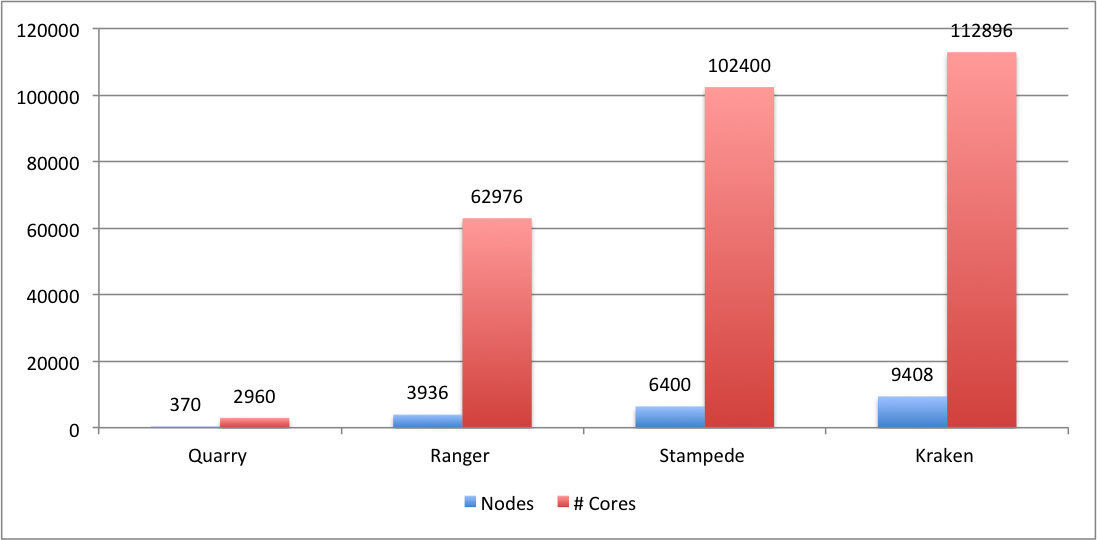
\includegraphics[width=0.49\textwidth]{figures/cores-nodes.png}
\caption{Mason and Quarry are IU resources, while Ranger, Stampede and Kraken are XSEDE resources. The graph shows the large change in the size of the machines that the users experience when they move to XSEDE.  }
\label{fig:scaling}
\end{figure}

\subsection{Research Plan}\label{sec:plan}

%\abhi{change the following paragraph to indicate what we actually did and why. i.e. doing more kbp/genome and may be more genomes}

As a first step, we applied for a startup allocation on Ranger and Kraken to
benchmark the mlRho application. We also planned to use the startup allocation to conduct a scaling study. A service
unit in XSEDE is defined as one core hour on a machine. It became apparent that conducting the study for
all 70+ genomes would require at least 15 million SUs. However, given that the researchers
are new to the XSEDE ecology and this is the first time they are applying for a large scale allocation, we
wanted to stay under the 5 million SU mark. To do this, we pared down the list to 46 diploid eukaryotic
genomes. We initially determined to measure 100 kilo basepair (kbp)
distances to limit the number of SUs required. Given that in eukaryotes, recombination
rates range between 0.001$-$1 event per Mbp~\cite{annurev-genom-082410-101412}, a 100 kbp window across a
genome provides a good basis for capturing the signature of crossover events that occur 1 or 2 times per
chromosome arm per meiotic event.

%Our approach to linkage analyses requires diploid genomes that have not been intentionally inbred (e.g., some
%plant genomes) or sequenced from several individuals. The list of 46 species were carefully selected from
%several important taxonomic groups to represent organisms with different ecology, population history, and
%reproductive strategies (e.g., asexual vs. sexual). This list thus constitutes a core dataset to develop a
%broad survey of linkage disequilibrium, population recombination rate, and population histories across
%eukaryotes. Furthermore, we have included genomes from multiple individuals for both {\it Daphnia pulex} and
%humans to explore intraspecific differences in linkage patterns and population histories.

\subsection{Scaling Up to XSEDE}
\label{sec:tests}

For some time the researchers had been running the mlRho code on local IU resources serially, by requesting
one compute-node at a time. Given that the IU resource, Quarry, had a serial queue that placed multiple serial jobs from
a single user on the same node, this was a feasible course. Unfortunately, most of the major XSEDE resources do
not provide such a high throughput queue. The users are charged for the whole node, irrespective of the number
of cores their job actually utilizes. Moreover, the larger machines are configured for highly parallel jobs and
the schedulers are configured to prioritize larger jobs. Many XSEDE centers have established workarounds for this
problem by providing users with wrappers and other software which bundle many serial jobs into larger jobs. We decided to use Ranger for our project, as BigJob was still in an experimental state on Kraken at this point. 


\subsubsection{SAGA BigJob framework}
\label{sec:bigjob}

We used the SAGA BigJob to bundle our serial mlRho simulations. We have integrated mlRho with
BigJob and conducted several experiments on Ranger and Stampede which have shown good performance and
scalability.  BigJob is a pilot-job tool available on many XSEDE resources such as Kraken, Ranger, and
Lonestar. Many researchers have successfully used BigJob~\cite{saga_bigjob_condor_cloud} to bundle hundreds of smaller jobs into larger, more manageable groups of jobs~\cite{Luckow:2008fp, async_repex11}.

BigJob maintains the list of processors allocated after the job request becomes active. The
user can design the BigJob to assign these processors to start and manage smaller jobs. The main benefit of doing this is that instead of submitting
thousands of single core job requests to the queue, we can submit hundreds of large job requests ($\approx$
500 to 5000 cores) to the queue. This reduces the overall number of job submissions to the queue and thereby,
to some extent, time spent waiting in the queue. This job size is also more appropriate for many of the XSEDE
machines.\\
\\



\begin{figure*}[t] %[h!] % t=top, b=bottom, h=here, p=separate page
\centering
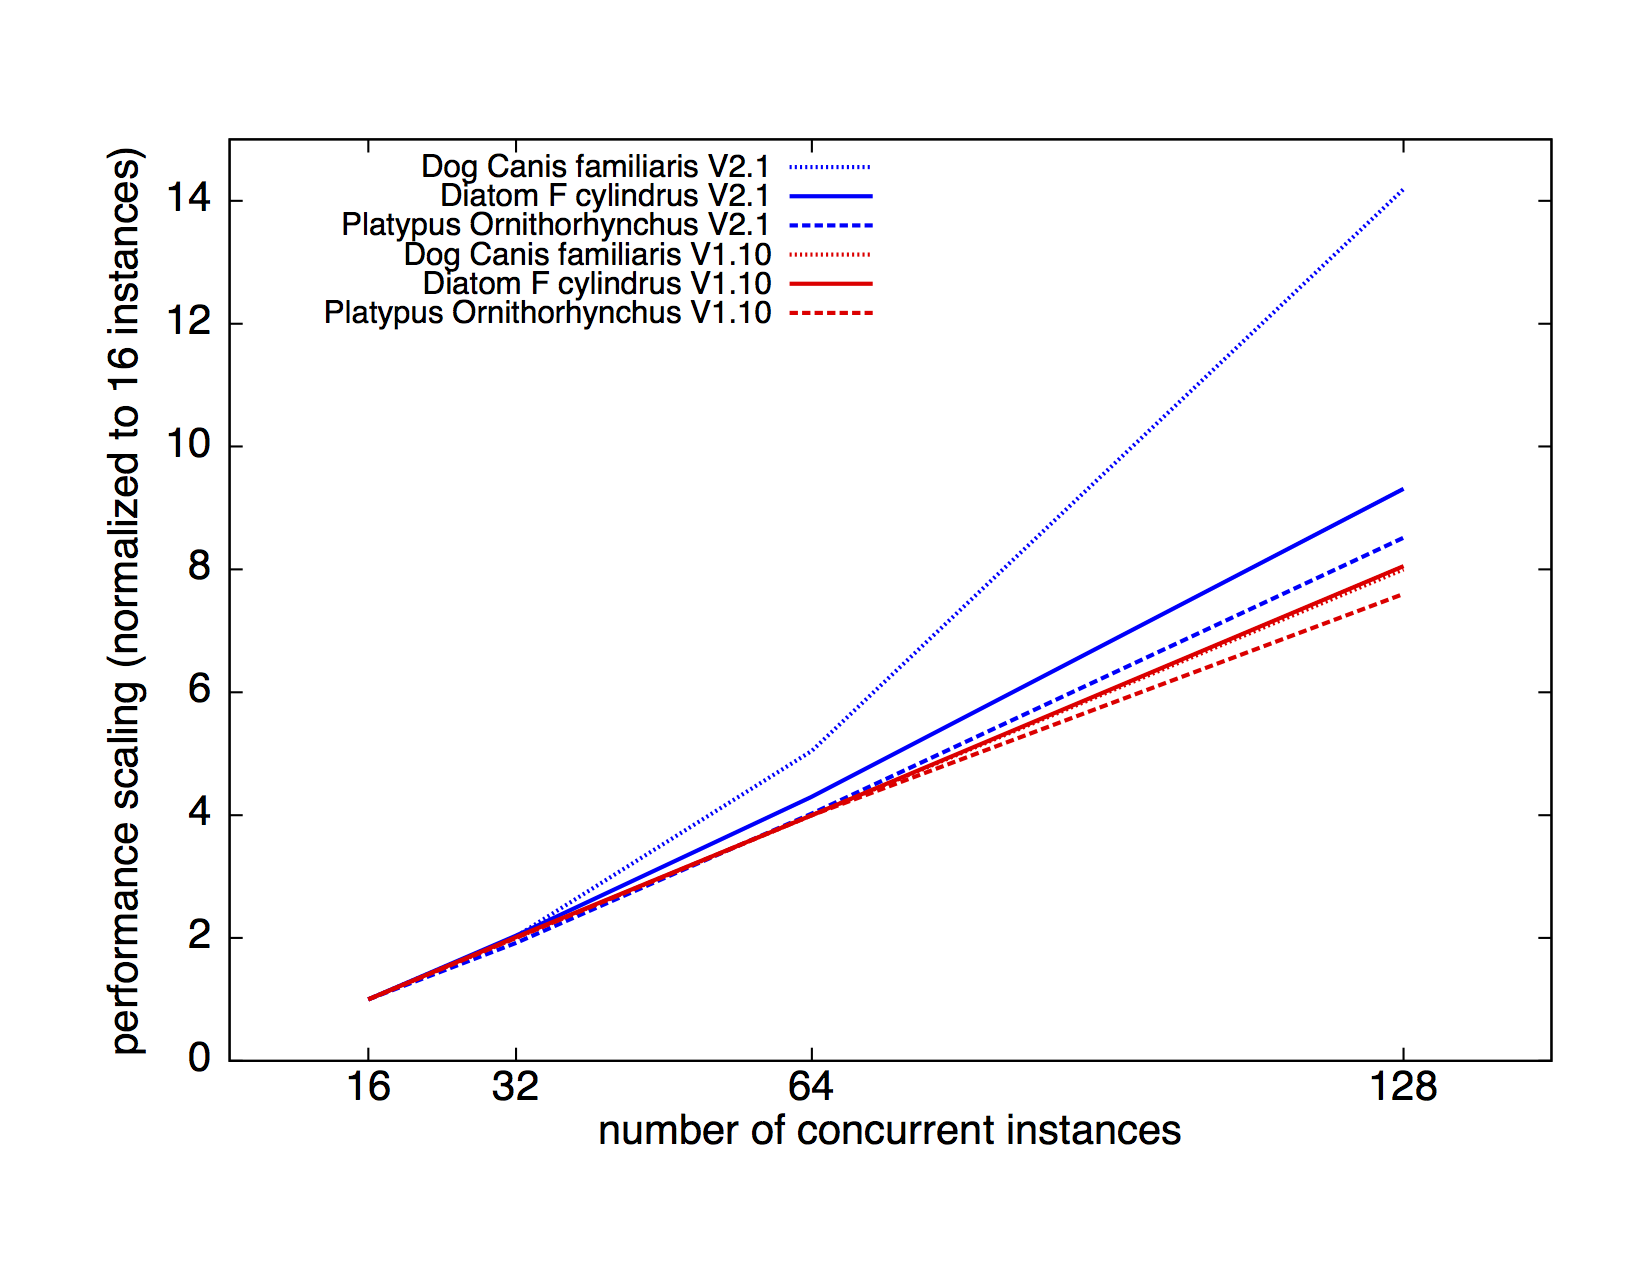
\includegraphics[width=0.78\textwidth]{figures/bj-scaling.png}
\caption{After running 16, 32, 64 and 128 instances of mlRho concurrently using BigJob on Ranger and Stampede with versions 1.10 and 2.1, respectively, we see that amount of work done increases nearly linearly with the number of instances of mlRho. The y-axis shows the total distance travelled by all the instances put together and normalized to 16 instances. The x-axis shows the number of concurrent mlRho processes running. }
\label{fig:bj-scaling}
\end{figure*}

\subsubsection{mlRho Scalability tests}
\label{sec:scalability}
We used the BigJob installation already in place on Ranger. The major focus of our tests was to discover how
mlRho scaled when we increased the number of concurrent mlRho processes. We took three different organisms
based on the size of their genome: a small genome, {\it F. cylindrus} (diatom), a medium genome, {\it
P. ornithorhynchus} (platypus), and a large genome, {\it C. familiaris} (dog). Data sizes are provided in Table
\ref{table:cache_comp}. We ran the mlRho program with each of these genomes starting with 16 concurrent mlRho
instances reading from the same data file. We let the processes run for 24 hours and measured how many
distances were computed in aggregate. It was clear that the distance travelled per second directly depended on the size of the genome.
\begin{table}[h]
\centering
\begin{tabular}{|p{3cm}|c| c |c  |     } \hline
{ Organism Type	}	& { Size of profile}& \multicolumn{2}{|c|}{{ Distance/sec} } \\ \hline
	& { (GB)}  & { V 1.10} & { V 2.1} \\ \hline
{ {\it F. cylindrus (diatom)} } & { 0.72  }& { 0.0034} & { 0.323} \\ \hline
{ {\it P. ornithorhynchus (platypus)} } & { 11 } &{ $2.3{\times}10{-4}$ }&  { 0.020} \\ \hline
{ {\it C. familiaris (dog)} } & { 31} & { $8.1{\times}10^{-5}$} & { 0.005} \\
\hline
%Intel & 405 & 388 & 364 & 346\\
%\hline
%PGI &418 & N/A   & N/A &N/A\\
%\hline

\end{tabular}
\caption{The table lists three organisms which were chosen to represent profiles of different size. The second column shows the size of the profile in gigabytes. The third column shows the distance travelled per second by V1.10 and V2.1 on one core on Ranger and Stampede, respectively. The rate of distance is a function of the size of the genome.  } 
\label{table:cache_comp}
\end{table}

 We repeated this for each of the genomes with 32, 64 and 128
concurrent instances. The results are shown in Figure~\ref{fig:bj-scaling}. Figure~\ref{fig:bj-scaling} shows that the distance traveled, irrespective of the genome, size, and the number of concurrent instances, increases
nearly linearly with number of concurrent instances being run. We have verified this behavior on Stampede with
an optimized version of mlRho (V2.1) and obtained similar results. We are unable to repeat this scaling study on
Ranger with the improved version of mlRho as Ranger has since been decommissioned.

%Table~\ref{table:bj_runs} shows the distance traveled by each instance in 24 hours for different genomes. This also shows that the distance traveled is a function of the size of the genome data file. As the reader can observe, distance traveled is directly proportional to the size of the genome data file. We were able to estimate the SUs required per distance per GB of genome data file using each of the three genomes -- all three estimates are nearly identical. Based on these results, we are confident that we can scale up to more than 1000 concurrent instances per genome using BigJob.

%\begin{figure*}[htp]
%  \centering
%
%
%  \subfloat[Scaling characteristics of version 1.10 on Ranger ]{\label{fig:ranger}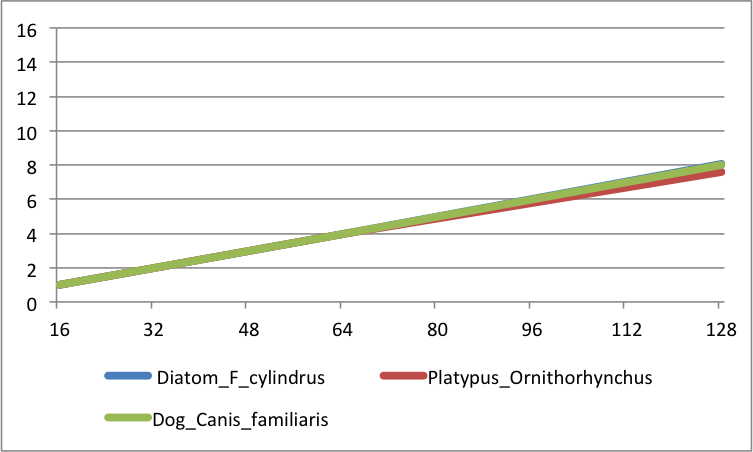
\includegraphics[width=80mm]{figures/scaling-ranger.png}}
%  \subfloat[Scaling characteristics of version 2.1 on Stampede]{\label{fig:stampede}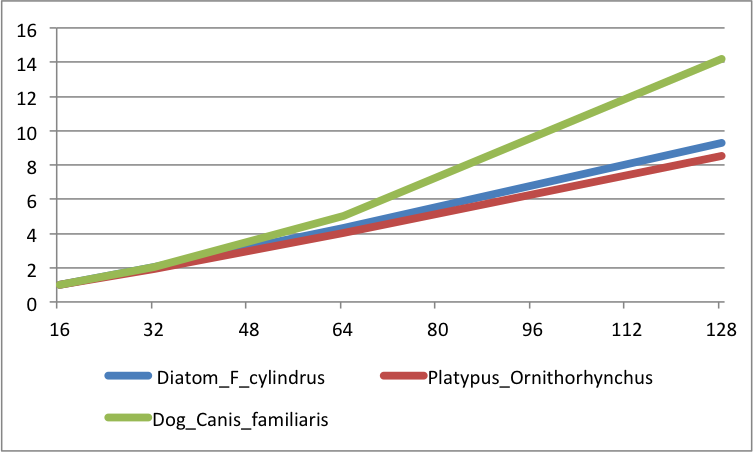
\includegraphics[width=80mm]{figures/scaling-stampede.png}}
%  \label{fig:bj-scaling}\caption{After running 16, 32, 64 and 128 instances of mlRho concurrently using BigJob on Ranger and Stampede with versions 1.10 and 2.1, respectively, we see that amount of work done increases linearly with the number instances of mlRho. The Y-Axis shows the total distance travelled by all the instances put together and normalized to 16 instances. The X-Axis shows the number of concurrent mlRho processes running. }
%\end{figure*}

\subsection{XSEDE Allocation}
%\abhi{notes: startup alloc help -- CBridgers's help needed, scalability tests, etc}

In general, obtaining an XSEDE allocation with sufficient SUs is an important step in the process of executing
a computationally intensive research plan. Even to someone who has a computer science background, writing a
successful XSEDE proposal is not a trivial task. The computational justification for the allocation needs to
be concrete and this is especially true if the request is for more than a few million SUs. XSEDE
allocation committees are routinely faced with the fact that the machines are oversubscribed by a factor of 2:1.

We believe that allocation proposal preparation is one key area where users new to XSEDE need significant
help. In the case of the mlRho project, research staff from the Indiana University Pervasive Technology
Institute (PTI) helped biologists to prepare an allocation proposal. We started by requesting startup
allocations on Ranger and Kraken. We benchmarked mlRho on a single core on Ranger and Kraken. We then did a
scalability study as described in section \ref{sec:scalability}. It is important to accurately estimate and
justify the total number of SUs that we request from XSEDE.  We usually also need to justify the science, but if the
research is supported by a current grant award from a federal science agency, further justification is not
needed. Given that we are requesting shared resources, it is important that we make an effort to analyze and
optimize our code. This reduces our own usage time and also turnaround time. We began to look into code
optimization shortly after submitting the proposal. Our efforts on the analysis and optimization of the code
is discussed in section \ref{sec:optimization} in more detail.


\subsubsection{Design of Experiments}

We have carefully constructed a detailed plan on how to proceed with our experiments. In section
\ref{sec:tests}, we showed that the mlRho code can scale to 128 processes, with each process reading from the
same file with no performance degradation. We estimated that we can feasibly scale up to $\approx$500
processes reading from the same data file, without noticeable performance degradation. By making multiple
copies of the data file, we could scale up to $\approx$5000 processes. Job requests of 5000 processes on
Ranger and Kraken are appropriate and we have not experienced extremely long wait times (more than 48 hours) with past BigJob experiments. We proposed that with this design, we could complete our analysis within four to five months from
the time of the allocation award. %This proposed framework was already working on Ranger, and was in the
%process of being implemented on Kraken.

In our initial testing of the three sample genomes, we worked out a few issues that could have affected
scalability. One of those issues was data access and file striping. When we had scaled up to 128 cores we
noticed some intermittent I/O issues. Since all the concurrent instances read from a single file, if that file is
singly striped in a Lustre file system, it will introduce a large load on the Lustre servers. We have remedied
this issue by moving the data files to the scratch file system on Ranger and striping the data files 16
ways. While this only occurred with the larger (11 and 31 GB) data files, we are aware that this might limit
our scalability. In the future, if I/O becomes an issue for scalability, we plan to use multiple copies of the
same data file to prevent an excessive number of concurrent processes from reading from the same file at the
same time.


\section{Optimization of mlRho}\label{sec:optimization}
We can not stress enough how important it is for each and every user of a shared supercomputer to analyze and optimize their code. This is especially true in the case of users who develop their own code. Most community codes are analyzed and optimized by their developers. But still, it is not unusual to see a 10\% gain in performance just by moving from one compiler to another. Given that XSEDE distributes hundreds of millions of SUs every year, even a 10 or 20 percent improvement will save millions of SUs and lower queue waiting times. 
\\
\\

\subsection{Performance Analysis}\label{subsec:analysis}
%\subsection{Source-code Development and Optimization}
Following its initial release in 2010\cite{MEC:MEC4482}, mlRho is being developed through a collaboration
 of research labs at IU and the Max Planck Institute for Evolutionary Biology (MPI) in Germany.
 Following initial benchmarking and scalability
testing for an XSEDE allocation proposal, staff members from the IU Pervasive Technology Institute worked
together with the mlRho application developer at MPI to improve the serial performance of the code. As a result of the investigations by PTI and MPI,  a new version which is vastly more efficient and delivers much better performance when compared to
the original version has been released. While the work described in the previous sections could be addressed by the campus
bridging expert role, the analysis and optimization described in this section would most likely be associated with
the XSEDE ECSS team. In this particular case both roles were fulfilled by a single team member at PTI. However,
it is certainly possible that these two roles could be filled by different teams at different institutions.

\subsection{Implementation of  Performance Analysis Findings}
Research staff at PTI began code optimization with mlRho version 1.10. As a first step, we compiled
the code with compilers other than the standard GNU compiler. Both the
Intel and PGI compilers produced a runtime improvement of $\approx$10\% over the GNU compiler on Ranger, this
is a fairly typical result that the optimization team at PTI has seen in many instances. From this point we
determined that further improvements would most likely be gained by modifications to the source code. To
inform the core developer at MPI as to
where his efforts would be best spent, we conducted a detailed analysis of mlRho version 1.10 using
the Vampir toolchain. The analysis led the core developer to focus on two aspects of the code: data handling
and repeated computation. As to data handling, many profiles occur repeatedly in a data set. To address this,
an additional program, formatPro, was written to compress the raw profiles. The formatPro program reads profiles either from a text
file or from a BAM file, the standard format for distributing genome alignment files \citep{li09:seq}. 

This new method of data storage increased performance by more than a factor of two from version
1.16 to 1.21 (see Figure \ref{fig:stampede-bench}). The formatPro program writes a binary table of unique
profiles.
% \begin{lstlisting}
% /* write tag for recognizing file type */
% fwrite("sum",sizeof(char),3,profileF);
% /* note the number of profiles */
% fwrite(&numNode,sizeof(int),1,profileF);
% /* write the profiles */
% fwrite(profiles,sizeof(Profile),numNode,profileF);
% \end{lstlisting}
%where a profile is
% \begin{lstlisting}
% typedef struct profile{  
%   int profile[4];        /* profile               */
%   int n;                 /* number of occurrences */
% }Profile;
% \end{lstlisting}
The binary file can then be inspected using the program inspectPro.
% \begin{verbatim}
% inspectPro profileDb.sum | head -n 3
% #ID	Count	A	C	G	T
% 0	1411292	0	0	4	0
% 1	1410182	4	0	0	0
% \end{verbatim}
In addition to the profiles file, formatPro writes a binary file
listing the profile ID at every genome position.
% \begin{verbatim}
% inspectPro profileDb.pos | head -n 3
% #Pos	Pro
% 1	0
% 2	1
% \end{verbatim}
Finally, formatPro writes a binary file of the contig lengths.
% \begin{verbatim}
% inspectPro profileDb.con | head -n 3
% #ID	Length
% 0	434
% 1	32
% \end{verbatim}
The mlRho program can then read the profiles from the files produced by formatPro.
% \begin{lstlisting}
% /* read first three characters */
% fread(&tag,sizeof(char),3,fp);
% /* read the number of profiles */
% fread(&numProfiles,sizeof(int),1,fp);
% /* allocate space for profiles */
% profiles = (Profile *)malloc(numProfiles*sizeof(Profile));
% /* read profiles */
% for(i=0;i<numProfiles;i++)
%   fread(&profiles[i],sop,1,fp);
% /* make profiles available for further computations */
% setProfiles(profiles);
% setNumProfiles(numProfiles);
% \end{lstlisting}
The profiles are read individually rather than in a single
step, because we found that this improved stability on the Lustre filesystem.
 The improvement in data handling introduced with these changes resulted in an overall speedup of the
serial code by a factor of 2-4X. The next focus was to look at the repeated computation that occurred in the
mlRho program. 

In the version 1.10 of the mlRho program, the likelihood computation iterated over all positions. By
introducing several improvements in how the likelihoods are calculated, the program now iterates over a much
smaller number of unique profiles. This improvement can be noticed in Figure \ref{fig:stampede-bench} between
versions 1.21 and 1.23.
% \begin{lstlisting}
% for(i=0;i<numProfiles;i++){
%   /* likelihood given that position is homozygous */
%   lOneLoc = lOne(coverages[i],profiles[i].profile,ee);
%   /* likelihood given that position is heterozygous */
%   lTwoLoc = lTwo(coverages[i],profiles[i].profile,ee);
%   l = lOneLoc * (1.0 - pi) + lTwoLoc * pi;
%   likelihood += log(l) * profiles[i].n;
% }
%\end{lstlisting}
In addition, the unique likelihoods are now written to disk for future reference.
% \begin{lstlisting}
% /* write tag for identifying file */
% fwrite("lik",sizeof(char),3,fp);
% /* write size of data structure */
% fwrite(result,sizeof(Result),1,fp);
% /* save number of profiles considered */
% np = getNumProfiles();
% fwrite(&np,sizeof(double),1,fp);
% /* write likelihoods given homozygosity */
% fwrite(getLones(),sizeof(double),getNumProfiles(),fp);
% /* write likelihoods given heterozygosity */
% fwrite(getLtwos(),sizeof(double),getNumProfiles(),fp);
% \end{lstlisting}

In the disequilibrium analysis of the 1.10 version, the single-site likelihoods were recomputed for every
step. To improve efficiency, they are now either read from disk or stored after the first pass across the
data. In addition, we noticed that by ignoring the order of two profiles, we could halve the number of
distinct profile pairs stored in a search tree. The likelihood computation during traversal of this tree is
now based entirely on precomputed probabilities.
% \begin{lstlisting}
% void traverse(int a, Node *np, double h0, double h2, double complementHalf){
%   if(np != NULL){
%     traverse(a,np->left,h0,h2,complementHalf);

%     b = np->key;
%     li = h0*lOnes[a]*lOnes[b]
%        + h2*lTwos[a]*lTwos[b]
%        + complementHalf*(lOnes[a]*lTwos[b]+lTwos[a]*lOnes[b]);
%     likelihood += log(li) * np->n;

%     traverse(a,np->right,h0,h2,complementHalf);
%   }
% }
% \end{lstlisting}
% where \ty{h0} is the probability of observing a homozygous pair and
% \ty{h2} the probability of observing a heterozygous pair. These two
% quantities are a function of the rate of recombination. The variable
% \ty{complementHalf} simply stores $1-(\ty{h0} + \ty{h2})$.
The combination of better data handling and careful avoidance of repeated computation led to an overall 50-fold
speedup of mlRho without increasing the minimal memory 
requirement observed in version 1.10.

\begin{figure} %[h!] % t=top, b=bottom, h=here, p=separate page
\centering
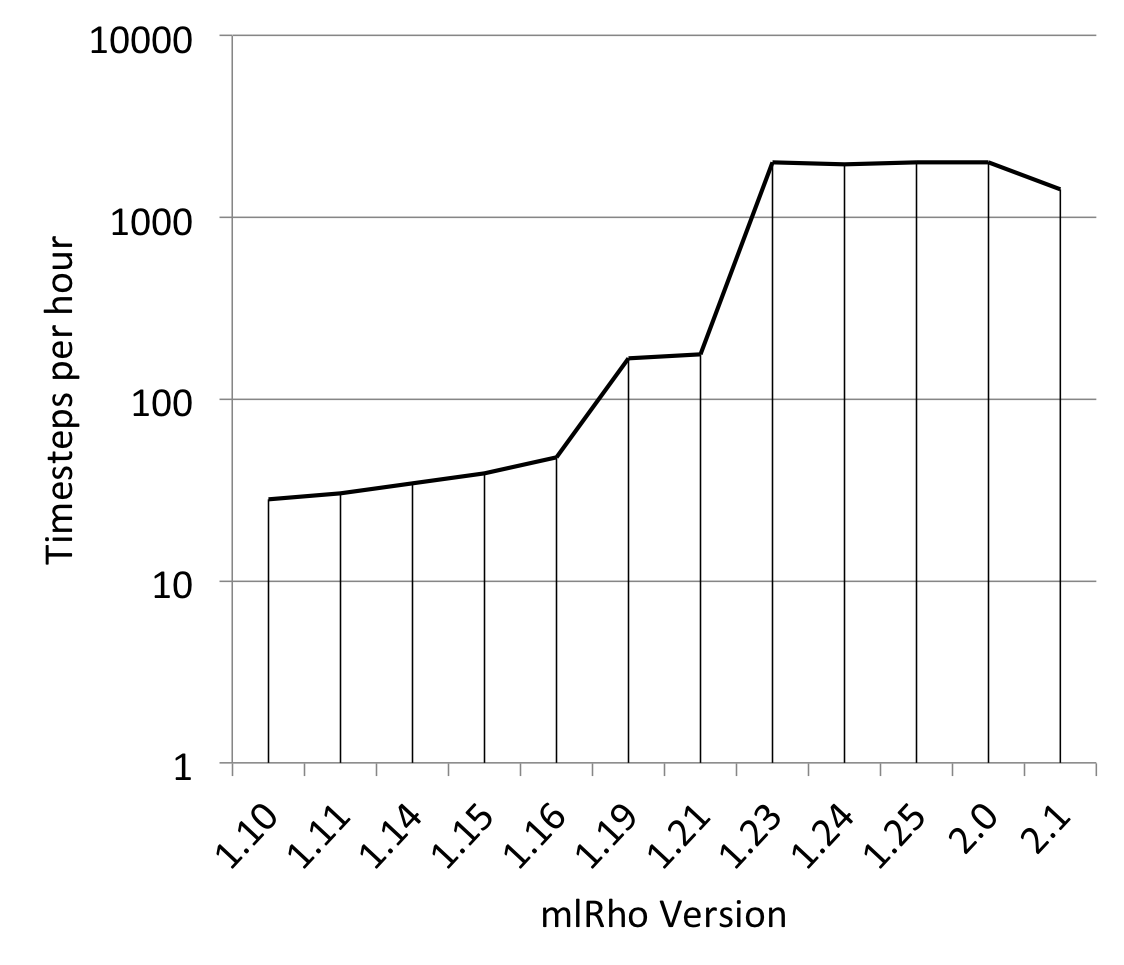
\includegraphics[width=0.48\textwidth]{figures/mlrho-benchmarks.png}
\caption{The graph shows the different versions of mlRho benchmarked on a single core on Stampede. The y-axis shows the change in time steps per hour with respect to version 1.10 in logarithmic scale. Compared to version 1.10,  2.1 is more than 50 times faster. }
\label{fig:stampede-bench}
\end{figure}

%\begin{table}
%\centering
%\begin{tabular}{| l  | l  | l  | l  | l  | l  | l  |} \hline
%	&Ranger & \multicolumn{3}{|c|}{Mason}\\ \hline
%	& 1.11  & 1.10&1.11 & 1.14\\ \hline
%GNU & 450 & 508 & 414 & 394   \\
%\hline
%Intel & 405 & 388 & 364 & 346\\
%\hline
%PGI &418 & N/A   & N/A &N/A\\
%\hline
%
%\end{tabular}
%\caption{\abhi{placeholder}The table shoes mlRho runtimes on different machines with different compilers. The runtimes are in seconds. Compiling with the Intel compiler gave us a 10\% speedup compared to GNU/PGI compilers on Mason and Ranger. Future work could include building GSL with Intel compilers.   } 
%\label{table:cache_comp}
%\end{table}

% \subsection{Code Validation}
% To determine the accuracy of the revamped mlRho, we simulated sequencing data with known mutation and
% recombination rates. Figure~\ref{fig:test}A shows that the mutation rate is accurately estimated even if
% exceeded by the error rate. Similarly, Figure~\ref{fig:test}B shows that the recombination rate is slightly
% underestimated if the mutation rate $\theta=10^{-2}$ and $\rho=10^{-2}$ or $\rho=10^{-3}$. However, the
% combination of low mutation and recombination ($\theta=\rho=10^{-3}$) gives very noisy results, demonstrating
% the method's limit of resolution.

% \begin{figure*}
%   \begin{center}
% \unitlength1in
% \begin{minipage}{0.45\linewidth}
% \centering
% 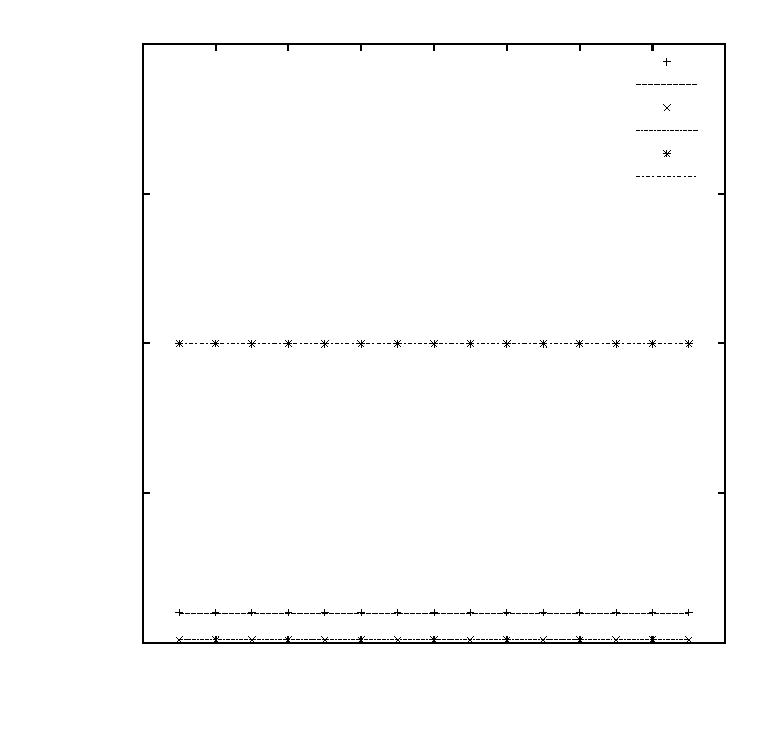
\includegraphics{figures/theta}
% \end{minipage}
% \begin{minipage}{0.45\linewidth}
% \centering
% 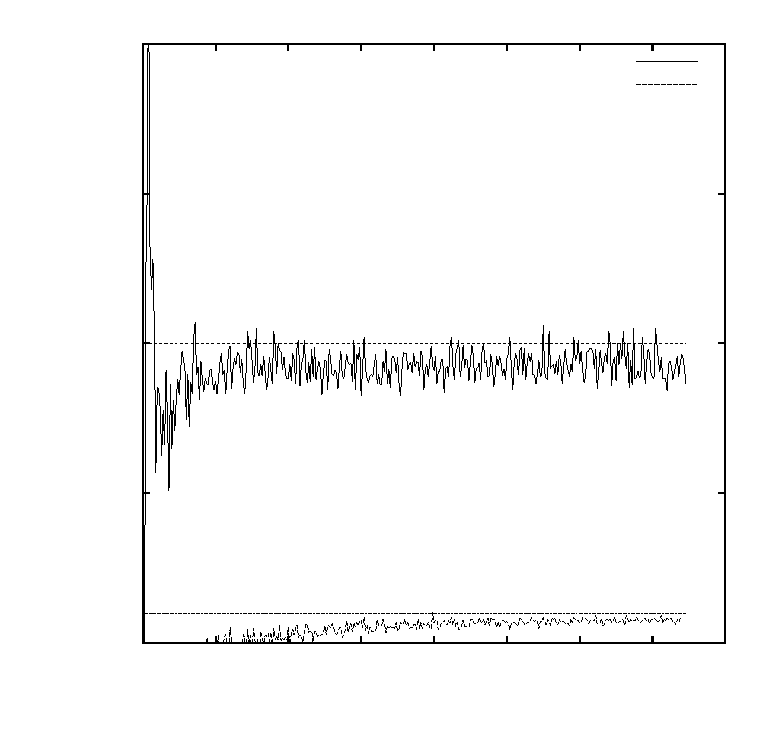
\includegraphics{figures/rho}
% \end{minipage}

% \caption{Testing the accuracy of mlRho. \textbf{A}: The mutation
%   rate estimator, $\hat\theta$, as a function of the sequencing error
%   rate, $\epsilon$; sequence length: $10^8$. \textbf{B}: The
%   recombination rate estimator, $\hat\rho$, as a function of pairwise
%   distance; the data set consists of 1000 pairs of 100kb sequences
%   with $\theta=0.01$ and $\epsilon=10^{-4}$; horizontal lines:
%   expected value. Coverage: 10.}\label{fig:test}
%   \end{center}
% \end{figure}

\section{User Experience, Preliminary Science Results, and Future Work}\label{sec:results}
\subsection{User Experience}
Overall the end user experience of migrating from the relatively modest Quarry and Mason local clusters to the
much larger Ranger resource on XSEDE was a smooth transition. This was mostly due to two factors, the
first of which was the similar computational environment on campus and XSEDE resources. We were able to
transfer all of the input data files from campus resources to XSEDE resources via the
XSEDE network using standard transfer mechanisms like \texttt{scp}. Since both the campus resources and Ranger and
Stampede at TACC use a variant of the modules software environment management system, replicating the software
environment on XSEDE resources was a simple matter of finding and loading the correct modules. Although the
scheduling systems used on the campus resources and XSEDE resources were different (TORQUE vs. SGE), there were
enough similarities and documentation on converting submission scripts and made the transition relatively
easy. 
 
The other factor in simplifying  the transition was the use of the BigJob framework coupled with the
consultation advice from the PTI staff. The initial transition to running mlRho in a massively parallel
way on Ranger was fairly straightforward (mainly due to the embarrassingly parallel nature of the problem),
and produced excellent throughput. Using BigJob to run thousands of mlRho processes was not without
issues, though. Without the aid of the PTI staff,
working effectively on Ranger and Stampede would have been extremely challenging. 
%\abhi{rewrite some of Sen's problems in the following paragraph with the actual issues and how  we resolved them}.
\subsubsection{Technical Issues }

The initial benchmarking and scaling tests that we did for the allocation proposal progressed smoothly. But as with any research project, we ran into many technical challenges when we started running experiments at scale on Ranger. There were scaling issues, problems with BigJob design/usage, and file system issues, and some of these led to the user getting banned from the system. Some of the major issues:
\begin{itemize}
\item We had to remain vigilant for issues related to the Lustre file system, given that hundreds of mlRho
  processes read from a single input file. We tried to address this problem by striping the directories
  containing the input files. TACC administrators advised us that striping the input files addressed the
  problem. We gradually scaled up our job size to 4000 cores on Ranger but this put excessive stress on the
  file system. Due to this issue, we decided to stay below 2000 cores. Another solution could be to have a
  different copy of the input file for every group of 500 mlRho processes.
\item The BigJob tool is and has been under active development. There were major design changes in process
  during the time that we started using it on Ranger. BigJob addresses a range of compute and data problems
  and multiple example scripts are available on its website. The initial version we deployed was not suitable for
  our task, which is bundling and running hundreds of serial jobs, and hampered performance. 
\item Another potential issue with BigJob is that the master process needs to be active from the time the job
  is submitted until the end of the job. This means that BigJob needs to be active on the login node of the
  system and cannot be disconnected. Another solution to this issue is to run BigJob in a screen session or use another
  tool like nohup on the login node. In the end we were told not to run more than four interactive sessions at a time, which was less than optimal for our use case. This issue has now been resolved by the BigJob developers by removing this requirement.
\item We also had problems with some mlRho processes failing, which forced us to identify and re-run
  these jobs. This was a major problem, but with both mlRho and BigJob were rapidly evolving. This made it difficult to diagnose the issue.

\end{itemize}


%My experience with running mlRho analysis using Bigjob on Ranger consisted of two different phases in terms of
%the program performance. When we were developing this idea to use Bigjob to run the analysis in an
%embrassingly parallel way (prior to July 2012), the performance of Bigjob was excellent. All the multicore
%jobs were completed nicely. However, after the approval of our allocation in September 2012, Bigjob had been
%upgraded. There seems a number of issues with Bigjob. 

%First of all, the way Bigjob is run involves using the
%command nohup. As all the jobs are submitted on the login node of Ranger, it is required that no more than 4
%nohup commands can be run at one time. 

%It occurred a couple times that I submitted more than 4 bigjobs on the
%login node and my jobs were all suspended. Subsequently, I was banned from running the jobs. Unfortunately, I
%was not notified until I found all my jobs were not running for two to three days. This seems to me rather
%counter productive. 

%For my project, I need to submit ~100 multicore jobs (requiring on average 1024-4096
%cores) in total. I would like to have the capacity to submit a number of jobs in the queue and collect data
%when the jobs are done. 

%Assuming each job is done right, submitting four jobs at a time is not
%problematic. What is truly problematic is that I encountered a situation that many cores (up to 60\% of the
%cores) in the same job cannot finish the analysis properly, resulting many missing values. Finding out the
%missing values and creating new jobs will not necessarily solve the problem, because I often had cores not
%working properly in these new jobs.  

\subsection{Preliminary Science Results}
%note from Sen
The analyses we were able to perform on Ranger and Stampede provided an extensive amount of data that would
have been unimaginable with campus resources. We began our study planning to analyze 100,000
basepair distances per genome. However, with the optimized version of mlRho performing at more than 50
times the efficiency of the version we began with, we have now completed 10 times the work we had initially
planned. For many genomes we have been able to compute up to 1 million basepair distances, and we have been
able to investigate many more genomes than originally proposed. Results from the new data indicate that the
zygosity correlation at large distances deviates significantly from theoretical expectation. This finding has
prompted us to begin new simulation and theoretical work to explain the observed discrepancy between the
theoretical prediction and our ML measurements on actual data. We believe that these new data will provide 
insights into the evolution of a large number of organisms.


\subsection{Future Work}
We have begun initial work on deploying the mlRho program on the Intel Xeon Phi coprocessor boards
available on Stampede. Since the Phi runs an embedded Linux Operating System \cite{xeon_phi}, 
it is relatively easy to launch multiple copies of the mlRho binary on the Phi board, assuming
that the input data set can fit in the memory footprint of the Phi board. In our case we copied input data
sets to the Phi RAM disk and computed against this copy. Figure \ref{fig:mic-scaling} compares the performance
of a single Phi board on the {\it F. cylindrus (diatom)} genome with the scaling measurements presented in Figure
\ref{fig:stampede-bench}. Here we compare to the scaling numbers for the Stampede timings using version 2.1 of
the mlRho software. By using a relatively large number of processes, in this case 488, on the Phi board
we are to achieve throughput that is roughly equal to the throughput of the CPUs on two Stampede
nodes. We are currently focusing our efforts on integrating the Phi scripts into the BigJob framework and
adding the Phi workload to the CPU workload. While writing a script for the BigJob framework is fairly
straightforward, the challenge is in properly balancing the load between CPU and Phi, particularly when the
input data access patterns (i.e. the input I/O) is very different for the CPUs and the Phi board.
\begin{figure} %[h!] % t=top, b=bottom, h=here, p=separate page
\centering
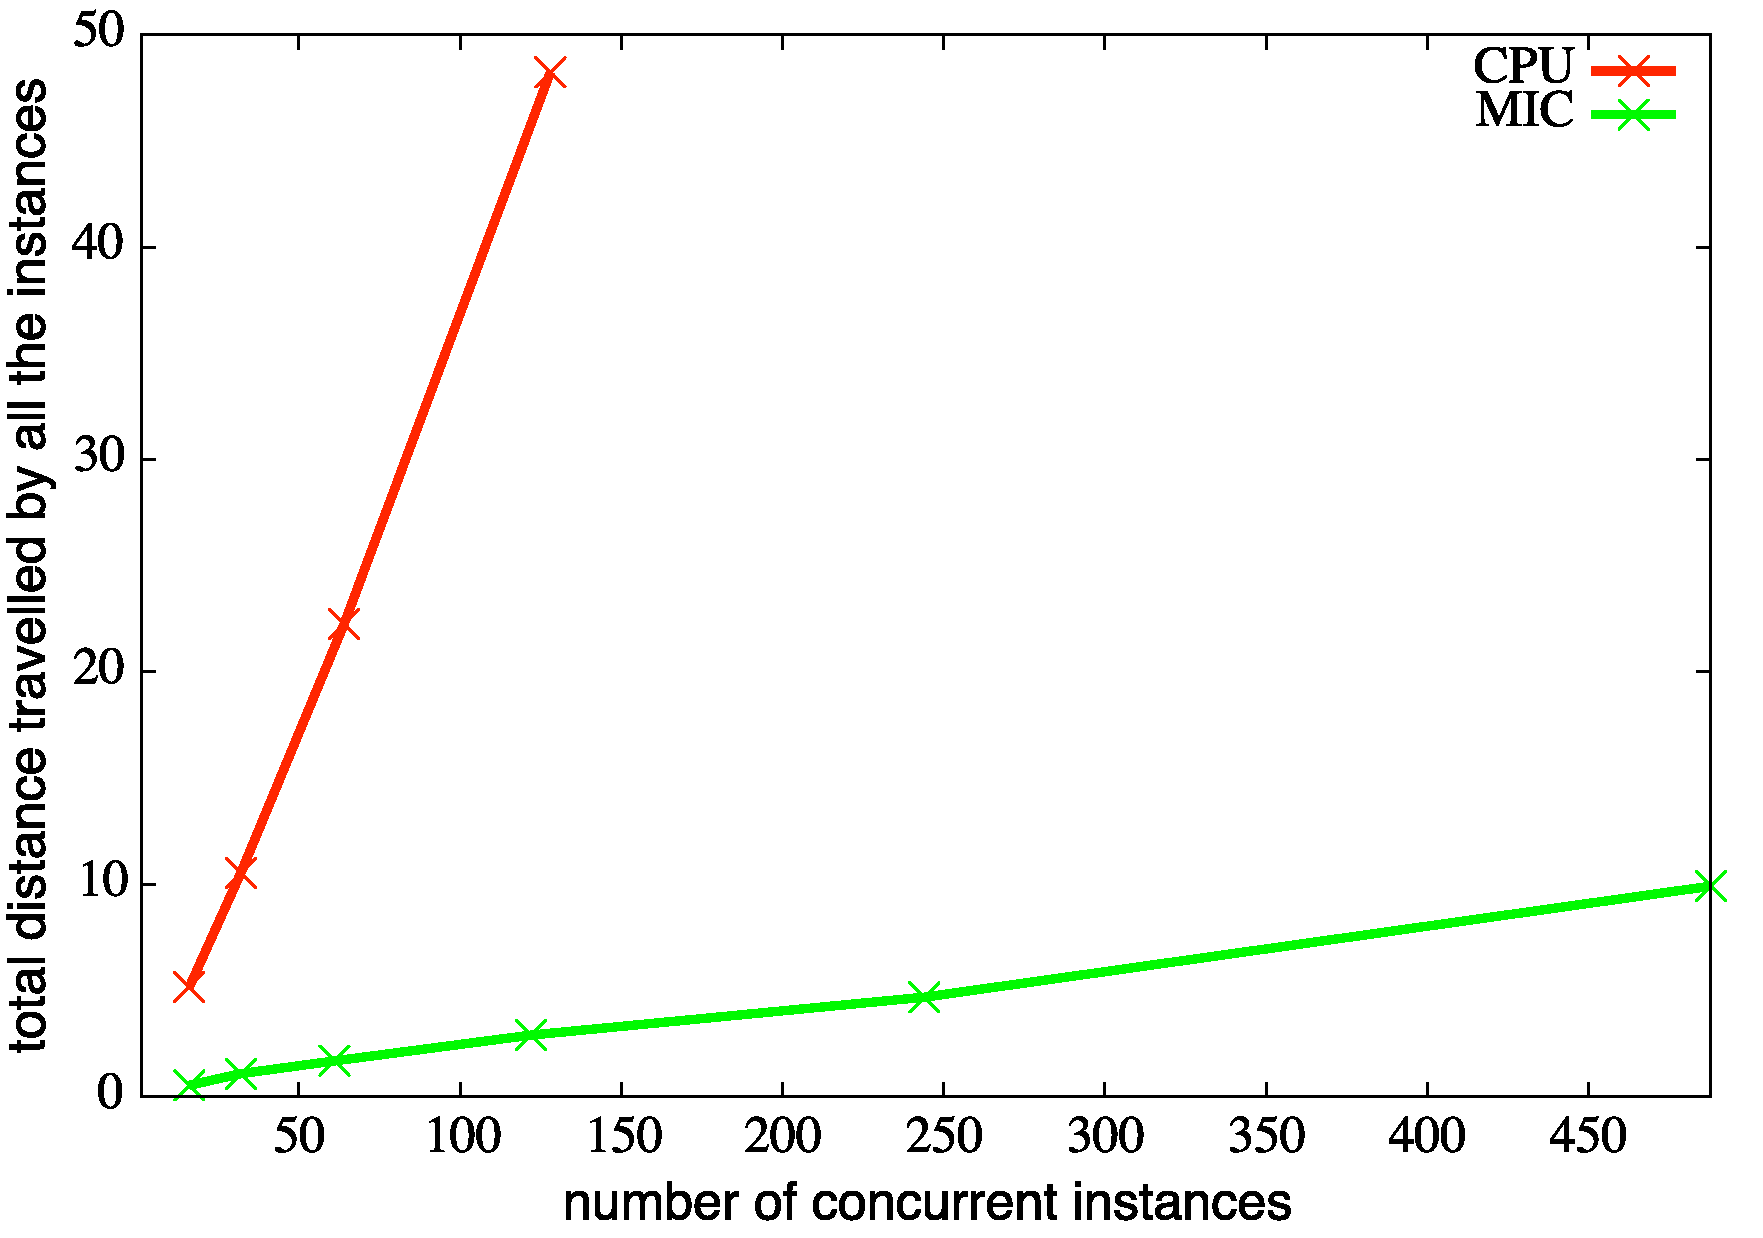
\includegraphics[width=0.42\textwidth]{figures/mic-scaling.pdf}
\caption{The graph compares the performance scaling behavior of mlRho on CPUs and Phis. Each mlRho process on a CPU was run on an individual core while multiple instances of mlRho were run on a single Phi. Four hundred and eighty-eight (488) mlRho instances on a single Phi gave us the same throughput as running 32 instances on two nodes of Stampede.  }
\label{fig:mic-scaling}
\end{figure}

\section{Conclusions}\label{sec:conclusion}

In all, the project of transitioning and scaling up mlRho workloads from campus computational resources
to XSEDE resources has been very successful, not only from the perspective of accelerating scientific
discovery, but also from the perspective of providing a real and useful example of the value of a campus
bridging expert. Through this project we have shown that a relatively small investment of effort by people
with the right mix of skills can make a big difference when transitioning from local
resources to XSEDE resources. We propose that XSEDE consider including the campus bridging expert role in more
of its supported projects, particularly those projects with PIs who are relatively new to high performance
computing concepts like batch scheduling, application scalability, and high performance file systems. As the
mlRho software continues to be improved and applied to more data sets, we hope to continue the excellent
synergistic relationship between domain scientists, computer scientists, and cyberinfrastructure
professionals.


%ACKNOWLEDGMENTS are optional
%acknowledgements -- xsede alloc, tacc people, saga team etc. 
%figure placement
\section{Acknowledgments}
We would like to thank C. Stewart for his insightful comments on the initial manuscript. We would also like to thank Y. El Khamra at TACC and the SAGA-BigJob team at Rutgers University for their help with technical issues. This work funded in part by NSF grants NSF EF-0827411 and NSF DEB-1257806. This work was
supported by XSEDE allocation TG-MCB120162. This research was also supported in part by the Pervasive
Technology Institute Initiative. The Pervasive Technology Institute Initiative of Indiana University is funded
by Lilly Endowment, Inc.
%
% The following two commands are all you need in the
% initial runs of your .tex file to
% produce the bibliography for the citations in your paper.
\bibliographystyle{unsrtnat}
\bibliography{xsede13}  % sigproc.bib is the name of the Bibliography in this case
% You must have a proper ".bib" file
%  and remember to run:
% latex bibtex latex latex
% to resolve all references
%
% ACM needs 'a single self-contained file'!
%
%APPENDICES are optional
%\balancecolumns
\end{document}
